\documentclass[a4paper]{article}
\usepackage[utf8]{vntex}
\usepackage[left=2.5cm,right=2.5cm,top=2cm,bottom=3cm]{geometry} 
\usepackage{graphicx} 
\usepackage{amsmath}
\usepackage{algorithm}
\usepackage{algpseudocode}
\usepackage{listings}
\usepackage{makecell} 
\usepackage{geometry} 
\geometry{a4paper, margin=1in}
\usepackage{algorithm}
\usepackage{algorithmic}
\usepackage[ruled,vlined]{algorithm2e}
\usepackage{courier}
\usepackage{tabularx}
\usepackage{float}
\usepackage[table]{xcolor}
\usepackage{xcolor}
\usepackage{amsfonts}
\usepackage{amsmath}
\usepackage{pgf-pie}
\usepackage{longtable}
\usepackage{mdframed}
\usepackage{array}
\usepackage{tikz}
\usepackage{bm}
\usepackage{hyperref}
\usepackage{scrextend}
\changefontsizes{13pt}
\usetikzlibrary{calc}
\usepackage{fancyhdr}
\setlength{\headheight}{40pt}
\pagestyle{fancy}
\fancyhead{} 
\fancyhead[L]{
 \begin{tabular}{rl}
    \begin{picture}(25,15)(0,0)
    \put(0,-8){
\includegraphics[width=8mm, height=8mm]{LOGO HCMUT.png}}
   \end{picture}&
        \begin{tabular}{l}
                { \ttfamily TRƯỜNG ĐẠI HỌC BÁCH KHOA - ĐHQG-HCM}\\
  { \ttfamily  KHOA KHOA HỌC VÀ KỸ THUẬT MÁY TÍNH}
        \end{tabular}   
 \end{tabular}
}
\pagenumbering{gobble}
\setcounter{page}{1}
\pagenumbering{arabic}
\fancyhead[R]{
        \begin{tabular}{l}
                \tiny \bf \\
                \tiny \bf 
        \end{tabular}  }
\fancyfoot{} 
\fancyfoot[L]{\scriptsize \ttfamily \textbf{  Báo cáo BTL môn Mô hình hóa toán học - CO2011}}
\fancyfoot[R]{\scriptsize \ttfamily Trang \thepage /28}
\renewcommand{\headrulewidth}{0.3pt}
\renewcommand{\footrulewidth}{0.3pt}
\usepackage{indentfirst}

\begin{document}
\begin{titlepage}
   
\begin{center}
    \vspace{1pt}
    {ĐẠI HỌC QUỐC GIA THÀNH PHỐ HỒ CHÍ MINH}\\
    {TRƯỜNG ĐẠI HỌC BÁCH KHOA}\\
    \textbf{KHOA KHOA HỌC VÀ KỸ THUẬT MÁY TÍNH}
    \\   
\end{center}


\vspace{10pt}
\begin{center}
    
\includegraphics[scale=0.7]{LOGO HCMUT.png}
    
    \vspace{40pt}
\fontsize{17pt}{17pt}\selectfont 
\begin{center}
\begin{tabular}{c}
\multicolumn{1}{l}{\textbf{{\Large MÔ HÌNH HÓA TOÁN HỌC (CO2011)}}}\\
~~\\
\hline
\\
\multicolumn{1}{l}{\textbf{{\Large Báo cáo Bài tập lớn}}}\\
\\
\textbf{\textit{{\Huge “Cutting stock problem”}}}\\
\\
\hline
\end{tabular}
\end{center}
\end{center}

\vspace{15pt}

\vspace{2cm}

\begin{table}[h]
\centering
    \begin{tabular}{rl}
    \textbf{GVHD}:
    & TS. Lê Hồng Trang\\
    & ThS. Mai Xuân Toàn\\

    & \\
    \textbf{SV thực hiện}: &  Hoàng Quốc Việt -  2313890 \emph{- L06, \textbf{Leader}} \\
    &  Bùi Trần Duy Khang- 2311402 \emph{- L06}\\
    &  Lê Trọng Tín - 2313452 \emph{- L06}\\
    &  Nguyễn Minh Tuấn - 2313749 \emph{- L05}\\
    &  Nguyễn Khánh Trình - 2313637 \emph{- L05}
    \end{tabular}
\end{table}

\vspace{50pt}
\begin{center}
    {TP.HỒ CHÍ MINH, THÁNG 11/2024}
\end{center}
\end{titlepage}

\tableofcontents
\newpage

\lstset{
  basicstyle=\footnotesize\ttfamily,
  keywordstyle=\color{blue},
  commentstyle=\color{green!60!black},
  stringstyle=\color{red},
  breaklines=true,
  numbers=left,
  numberstyle=\tiny\color{black},
  numbersep=5pt,
  tabsize=2,
  language=C++,
  xleftmargin=11pt,
  xrightmargin=11pt,
  frame=none 
}

\section{Giới thiệu bài toán}
\subsection{Tổng quan vấn đề}
\hspace{11pt}
Cùng với sự gia tăng dân số thế giới, đời sống vật chất của con người ngày càng nâng cao. Điều đó dẫn đến nhu cầu sử dụng tài nguyên thiên nhiên ngày càng lớn. Chúng ta đã và đang chứng kiến sự cạn kiệt của tài nguyên thiên nhiên, đặc biệt là các nguồn tài nguyên không tái tạo được như khoáng sản. Để phát triển bền vững, việc sử dụng các nguồn tài nguyên này một cách có hiệu quả là vấn đề quan trọng của nhân loại. Trong các ngành công nghiệp hiện đại như chế tạo máy, xây dựng, dệt may có một yêu cầu đặt ra là cần phải cắt một mẫu vật liệu thô có kích thước cố định thành kích thước theo yêu cầu. Từ một lĩnh vực gồm nhiều bài toán là Cắt vật tư và Đóng hàng(Cutting \& Packing - C \& P), bài toán cắt vật liệu (Cutting stock problem) là chủ đề tìm hiểu của nhóm nghiên cứu lần này. 

\hspace{11pt}
Tùy thuộc vào kích thước của bài toán mà số chiều có thể là 1,2,3 hoặc lớn hơn. Trong phạm vi của bài báo cáo, nhóm nghiên cứu xin được trình bày về hướng tiếp cận cũng như giải thuật được áp dụng cho bài toán cắt vật liệu 2 chiều.

\subsection{Lịch sử hình thành}
\hspace{11pt}
Từ giữa thế kỷ trước đã có nhiều cách tiếp cận để giải các bài toán cắt vật liệu và đóng hàng được đề xuất. Công trình nghiên cứu cho chủ đề này do L.V.Kantorovich đưa ra vào năm 1939 khi ông đề xuất áp dụng các mô hình toán học. Các mô hình này được phát triển dưới dạng các bài toán Quy hoạch nguyên và được chỉ ra thuộc lớp các bài toán NP-hard. Tuy nhiên do tồn tại một vài nhược điểm như có nới lỏng liên tục yếu và tính đối xứng nên việc áp dụng chúng trong các bài toán thực tiễn tỏ ra không hiệu quả.
Vì đây là một bài toán quy hoạch nguyên và thuộc lớp NP-khó vì vậy không tồn tại thuật toán đảm bảo cho nghiệm tối ưu trong thời gian đa thức.


\subsection{Đánh giá sơ bộ}
\hspace{11pt}
Do tính khoa học cũng như thực tiễn cao của chủ đề này nên nó đã thu hút sự chú ý của rất nhiều nhà toán học, khoa học nhằm tìm ra giải pháp tối ưu cho một bài toán có quy mô lớn như vậy. 

\hspace{11pt}
Các phương pháp giải quyết các bài toán cắt vật liệu một chiều có thể được chia thành hai loại: (1) thuật toán chính xác (exact algorithm) và (2) thuật toán xấp xỉ (approximation algorithm). Thời gian thực hiện của một thuật toán chính xác sẽ tăng lên đến mức không thể
chấp nhận được nếu quy mô của bài toán lớn hơn.

\hspace{11pt}
Nhiệm vụ cần phải làm là cắt tấm vật liệu thô ban đầu theo đúng như kích thước yêu cầu và tối thiếu hóa được phần vật liệu dư thừa.

%///////////////////////////////////////////////////
% SECTION : GIỚI THIÊU CÁC THUẬT TOÁN PHỔ BIẾN /////
%///////////////////////////////////////////////////
\section{Giới thiệu các giải thuật phổ biến}
\hspace{11pt}
Như đẫ đề cập, bài toán cắt vật liệu cần được áp dụng cho một số lượng lớn các mẫu vật tư thô, khi đó thời gian tính toán (computational time) có thể tăng lên đến với tốc độ hàm mũ.

\hspace{11pt}
Để giải quyết vấn đề này, các nhà khoa học đã nghiên cứu và phát triển nhiều thuật toán khác nhau, bao gồm các thuật toán chính xác và thuật toán xấp xỉ. Thuật toán chính xác, chẳng hạn như quy hoạch động hoặc quy hoạch tuyến tính nguyên, có thể đảm bảo tìm ra lời giải tối ưu nhưng thường không khả thi khi đối mặt với bài toán có kích thước lớn do hạn chế về thời gian và tài nguyên tính toán.

\hspace{11pt}
Trong khi đó, các thuật toán xấp xỉ, bao gồm các thuật toán heuristic, cung cấp lời giải gần đúng với thời gian tính toán nhanh hơn nhiều. Một số thuật toán phổ biến trong nhóm này bao gồm First Fit Decreasing Height (FFDH), Next Fit Decreasing Height (NFDH), và các thuật toán dựa trên nguyên lý di truyền (genetic algorithms) hoặc tối ưu bầy đàn (particle swarm optimization). Các thuật toán này không chỉ giảm thiểu đáng kể thời gian tính toán mà còn đạt được hiệu quả sử dụng vật liệu tương đối cao, phù hợp với các bài toán thực tế trong công nghiệp.

\hspace{11pt}
Việc lựa chọn thuật toán phụ thuộc vào các yếu tố như độ phức tạp của bài toán, kích thước của dữ liệu đầu vào, và yêu cầu về hiệu năng. Sự kết hợp giữa các thuật toán và phương pháp nghiên cứu chuyên sâu cũng được sử dụng để cân bằng giữa thời gian tính toán và chất lượng lời giải. 
%///////////////////////////////////////////////////
% THUẬT TOÁN LẶP KẾT HƠP ///////////////////////////
%///////////////////////////////////////////////////
\subsection{Thuật toán lặp kết hợp - Iterative Combinatorial Algorithm}
\subsubsection{Phương pháp nhánh cận của Christofides và Whitelock}

Cho một tấm vật liệu \( A_0 = (L_0, W_0) \) với chiều dài là \( L_0 \) và chiều rộng là \( W_0 \). \( R = \{(a_1, b_1), ..., (a_m, b_m)\} \) là một tập hợp các hình chữ nhật cần cắt. Mỗi hình chữ nhật được đặc trưng bởi:
\begin{itemize}
    \item \( v_i \): giá trị của hình chữ nhật,
    \item \( l_i \): số lần xuất hiện tối đa trong mẫu cắt.
\end{itemize}

Mọi số liệu trong bài toán là số nguyên, các vết cắt thuộc loại \textit{guillotine} (chỉ cho phép cắt theo đường thẳng), và không cho phép xoay các hình chữ nhật. Mục tiêu của bài toán là tối đa hóa 
\[
z = \sum t_i v_i,
\]
với các ràng buộc:
\[
0 \leq t_i \leq l_i, i = 1,...,m,\quad t_i \in \mathbb{Z}^+, 
\]
và tồn tại chuỗi các vết cắt từ \( A \) để tạo ra \( t_i \) hình chữ nhật loại \( i \).

\hspace{11pt}
Thuật toán này gồm 2 bước, trước hết cần sinh cây chứa tất cả các vết cắt có thể và sau đó quét cây để tìm đáp án tối ưu nhất.

\hspace{11pt}
Mỗi nút trong cây đại diện cho một vết cắt khả thi. Trong quá trình tạo cây, các vết cắt đối xứng được loại bỏ. Ví dụ, cắt hình chữ nhật \( (p, q) \) tại điểm \( e \) đối xứng với việc cắt tại điểm \( p-e \). Những cặp đối xứng kiểu như vậy được loại trừ bằng cách chỉ phân tích các điểm \( x \leq \lfloor p/2 \rfloor \) và \( y \leq \lfloor q/2 \rfloor \). Các vết cắt lặp lại được loại bỏ bằng cách áp đặt thứ tự kế thừa: ví dụ, nếu cắt tại điểm \( x = a \), thì các vết cắt tiếp theo phải được thực hiện tại \( x \geq a \). 

\hspace{11pt}
Chỉ các vết cắt "chuẩn hóa" (normalized cuts) mới được xem xét (xem Hình~\ref{fig : branch and bound}), tức là tại các điểm là tổ hợp tuyến tính của kích thước các phần tử. Điều này giúp loại trừ việc cắt gây lãng phí bên trong mẫu.
\begin{figure}[H]
\centering
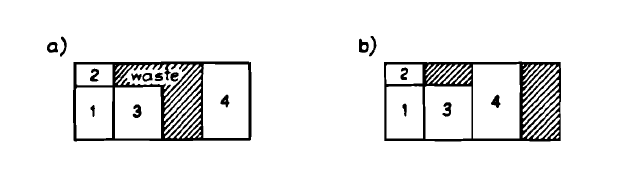
\includegraphics[width = 0.99\textwidth]{branch and bound.png}
\label{fig : branch and bound}
\caption{(a) Vết cắt không chuẩn hóa. (b) Vết cắt chuẩn hóa.}
\end{figure}

\hspace{11pt}
Các vết cắt khả thi của hình chữ nhật \( (p, q) \), dẫn đến các phần tử thuộc tập \( R \), là các phần tử của tập \( S_Q \) đối với các vết cắt theo chiều \( Y \), và tập \( T_P \) đối với các vết cắt theo chiều \( X \). Giờ đây, chúng ta mô tả cách tìm \( S_Q \) và \( T_P \).

\hspace{11pt}
Chúng được tìm theo cách tương tự. Hàm \( f_i(x) \) được sử dụng để tạo tập \( S_Q \). Hàm này có thể được tính đệ quy như sau (các hình chữ nhật được sắp xếp theo thứ tự giảm dần giá trị \( b_i \)):
\[
f_i(x) = \min\{f_{i-1}(x), \max\{b_i, f_{i-1}(x - j a_i)\}\}, \quad j = 1, ..., \min(l_i, \lfloor x / a_i \rfloor),
\]
với điều kiện \( x \geq a_i \).


\hspace{11pt}
Trạng thái của một nút trong cây được mô tả bởi danh sách \( L \) của các hình chữ nhật đã cắt trên đường từ gốc. Mỗi hình chữ nhật được biểu diễn trên danh sách này bằng vector \( (p, q, x, y) \), trong đó:
\begin{itemize}
    \item \( (p, q) \): kích thước của hình chữ nhật hiện tại,
    \item \( x, y \): các điểm mô tả các vết cắt tiếp theo nếu hình chữ nhật này được chọn.
\end{itemize}

\hspace{11pt}
Để tìm nghiệm tối ưu, giá trị cận trên của mỗi nút được tính thông qua phương pháp quy hoạch động (Dynamic programing) trên phiên bản đơn giản hóa của bài toán, không xét đén các giới hạn \(l_i\). Nếu giá trị \(z^*\) được tính toán tốt hơn nghiệm \(f\) đã tìm thấy trước đó, nghiệm hiện tại sẽ thay thế nghiệm cũ, và giải thuật tiêp tục với nút tiếp theo.

\subsubsection{Phương pháp kết hợp của Wang}
\hspace{11pt}
Thuật toán này là một thuật toán kết hợp, trong đó các mẫu cắt kiểu \textit{guillotine} được tạo ra bằng cách liên tục thêm các phần tử hoặc nhóm phần tử vào nhau. Các mẫu cắt này được chuẩn hóa tương tự như thuật toán trước đó. Để tránh sự tăng lên không kiểm soát của số lượng nghiệm từng phần, trong quá trình hiện thực sẽ loại bỏ các nghiệm vượt quá một tỷ lệ phần trăm xác định của diện tích tấm vật liệu hoặc vượt quá tỷ lệ phần trăm diện tích của nghiệm từng phần.

Ký hiệu:
\begin{itemize}
    \item \( S_k \): một nghiệm từng phần được tạo tại bước lặp thứ \( k \),
    \item \( F_k \): danh sách các nghiệm từng phần được tạo ra trong bước lặp \( k \),
    \item \( L_k \): danh sách các nghiệm từng phần được tạo ra đến bước lặp \( k \),
    \item \( \beta \): tham số loại bỏ, với \( 0 \leq \beta \leq 1 \).
\end{itemize}

Thuật toán của Wang có thể được trình bày như sau:
\begin{algorithm}[H]
\caption{Thuật toán Wang}
\KwIn{Tham số loại bỏ \( \beta \)}
\KwOut{Nghiệm tối ưu}
Khởi tạo: \\
          \( L_0, F_0 := R \);\\
          \( k := 0 \)\; \\
\While{\( F_k \neq \emptyset \)}{
    \( k := k + 1 \)\; \\
    \( F_k := \emptyset \)\; \\
    \textbf{sinh tất cả các nghiệm từng phần} \( S_k \): \textbf{thêm các phần tử từ} \( F_{k-1} \) \textbf{vào tất cả các phần tử trong} \( L_{k-1} \)\; \\
    \ForEach{\( S_k \)}{
        \If{\( S_k \) nằm trong tấm vật liệu\\
            \textbf{và} số lần xuất hiện của mỗi phần tử \( i \) trong \( S_k \) không vượt quá 1\\
            \textbf{và} phần lãng phí trong \( S_k \) không vượt quá \( \beta L_0 W_0 \)}{
            \( F_k := F_k \cup S_k \)\;
        }
    }
    \( L_k := L_{k-1} \cup F_k \)\;
}
\(M := k;\); \\
Chọn nghiệm tối ưu từ \( L_M \) với phần lãng phí nhỏ nhất\;
\end{algorithm}

\hspace{11pt}
\textbf{Tính chất tối ưu}: Nếu phần lãng phí của mẫu cắt tốt nhất không vượt quá \( \beta L_0 W_0 \), thì mẫu này là tối ưu (không tồn tại mẫu cắt nào khác có phần lãng phí nhỏ hơn).


\hspace{11pt}
\textbf{Cải tiến thuật toán}: Một phiên bản cải tiến của thuật toán áp dụng quy hoạch động để xử lý trường hợp số lượng phần tử không giới hạn. Điều này cải thiện cách tính toán phần lãng phí kỳ vọng cho nghiệm từng phần, giúp loại bỏ các nghiệm kém chất lượng từ sớm hơn.


%///////////////////////////////////////////////////
% SECTION : THUẬT TOÁN XẤP XỈ  /////////////////////
%///////////////////////////////////////////////////
\subsection{Thuật toán xấp xỉ - Approximation Algorithms}
\hspace{11pt}
Các bài toán tối ưu hóa không đảm bảo rằng sẽ đưa ra đáp án chính xác tuyệt đối mà cần yêu cầu phải tìm ra được đáp án gần đúng với đáp án chính xác nhất có thể trong thơi gian đa thức. Các thuật toán thực hiện được như mô tả trên được gọi là các thuật toán xấp xỉ (Approximation Algorithms) hay Thuật toán heuristic (Heuristic Algorithms).

\hspace{11pt}
Các giải thuật heuristic đầu tiên được đề xuất để giải các bài toán cắt vật liệu thường dựa trên các phương pháp tìm kiếm cục bộ như Next fit decreasing height (FFDH), First fit decreasing height (FFDH), \dots Nhóm báo cáo sẽ giới thiệu một vài thuật toán tiêu biểu và quan trọng nhất.

\hspace{11pt}
Không làm mất tính tổng quát, giả sử rằng chiều rộng của các tấm vật liệu cần cắt đã được cho trước, ta cần tối ưu hóa chiều dài của các tấm này. Với một tập \(L\) các hình chữ nhật đã cho và giải thuật xấp xỉ để tìm ra đáp an tối ưu cho bài toán là \(A(L)\) trong khi đáp án tối ưu là \(OPT(L)\). 

\hspace{11pt}
Ý tưởng chính của những phương pháp này là sau khi sắp xếp danh sách các thành phẩm theo thứ tự kích thước giảm dần, các phương án cắt được xây dụng theo các chiến lược khác nhau. 

Ta có \emph{tỉ lệ hiệu suất tuyệt đối (Absolute performance ratio)}:
\begin{center}
   \(A(L) \leq \alpha OPT(L)\) 
\end{center}


và \emph{tỉ lệ hiệu suất tiệm cận (asymptotic performance ratio)}:

\begin{center}
    \(A(L) \leq \alpha OPT(L) + \beta\)
\end{center}



\subsubsection{Next fit decreasing height (NFDH)}
\hspace{11pt}
Nếu không đủ không gian tại mức hiện tại (cao nhất) để đặt một mẫu vật liệu, thì tạo một mức mới (Đi theo chiều ngang từ trái qua).(Xem Hình~\ref{fig : next fit})

\begin{figure}[H]
\centering
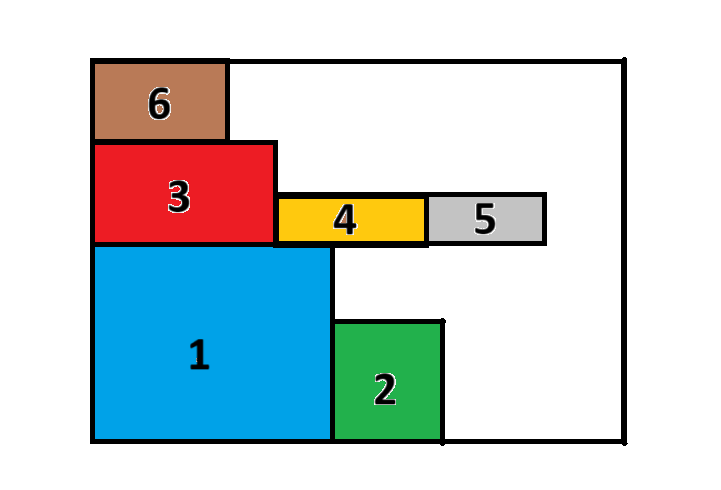
\includegraphics[width = 0.4\textwidth]{next fit.png}
\label{fig : next fit}
\caption{Kết quả mẫu minh họa thuật toán NFDH.}
\end{figure}

\subsubsection{First fit decreasing height (FFDH)}
\hspace{11pt}
Nếu như Next fit decreasing height(NFDH) ưu tiên đặt các mẫu đã được cắt theo chiều cao cho đến khi đạt mức tối đa, thì FFDH ưu tiên đặt các mẫu này vào các mức thấp nhất trước, nếu không đủ không gian thì lên mức cao hơn (Đi theo chiều dọc từ dưới lên). (Xem Hình~\ref{fig : first fit})

\hspace{11pt}
Tỉ lệ hiệu suất tuyệt đối của NFDH, FFDH lần lượt là 

\begin{center}
    \emph{\(NFDH(L) \leq  2 OPT(L) + 1\)} \\
    \emph{\(FFDH(L) \leq 1.7 OPT(L) + 7.3\)}
\end{center}

\hspace{11pt}
Và đối với các kích thước phần từ không được vượt quá \(\alpha\)
\begin{center}
    \(FFDH(L)\leq (1 + \frac{1}{m}) OPT(L) + (2 + \frac{1}{m}) \) với \(m = \lfloor1 / \alpha \rfloor\)
\end{center}
\hspace{11pt}
Đối với hình vuông
\begin{center}
    \(FFDH(L) \leq \frac{3}{2} OPT(L) + 2\)
\end{center}
\begin{figure}[H]
\centering
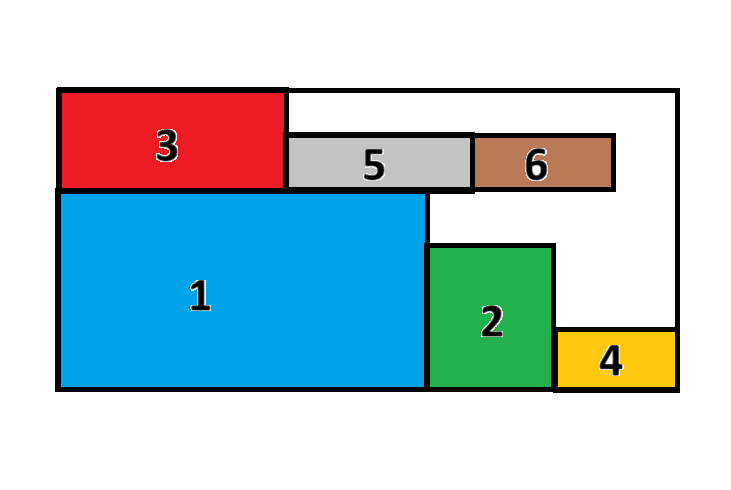
\includegraphics[width = 0.4\textwidth]{first fit.png}
\label{fig : first fit}
\caption{Kết quả mẫu minh họa thuật toán FFDH.}
\end{figure}


\subsubsection{Split fit (SF)}

\hspace{11pt}
Giả sử \(m \geq 1\) là số nguyên lớn nhất sao cho tất cả các hình chữ nhật có chiều dài không vượt quá \(l / m\). Danh sách các mảnh vật liệu đã cắt được sắp xếp theo thứ tự giảm dần của chiều cao. Chia \(L\) thành 2 danh sách \(L_1\) và \(l_2\):
\begin{itemize}
    \item \(L_1\) bao gồm các mảnh có chiều với chiều rộng lớn hơn \(1/(m + 1)\) 
    \item \(L_2\) bao gồm các mảnh còn lại.
\end{itemize}

\hspace{11pt}
Trước tiên, đặt các hình chữ nhật trong \(L_1\) bằng thuật toán FFDH. Sau đó di chuyển các lớp có chiều rộng lớn hơn  \((m + 1)/ (m + 2)\) xuống dưới các lớp có chiều rộng nhỏ hơn hoặc bằng \((m + 1)/(m + 2)\). Do đó một vùng rộng \(1 / (m + 2)\) sẽ được giải phóng. Đặt vào vùng này các mảnh trong danh sách \(L_2\) bằng thuật toán FFDH. Cuối cùng, đặt các hình chữ nhật \(L_2\) còn lại phía trên vùng cho \(L_1\).

\begin{figure}[H]
\centering
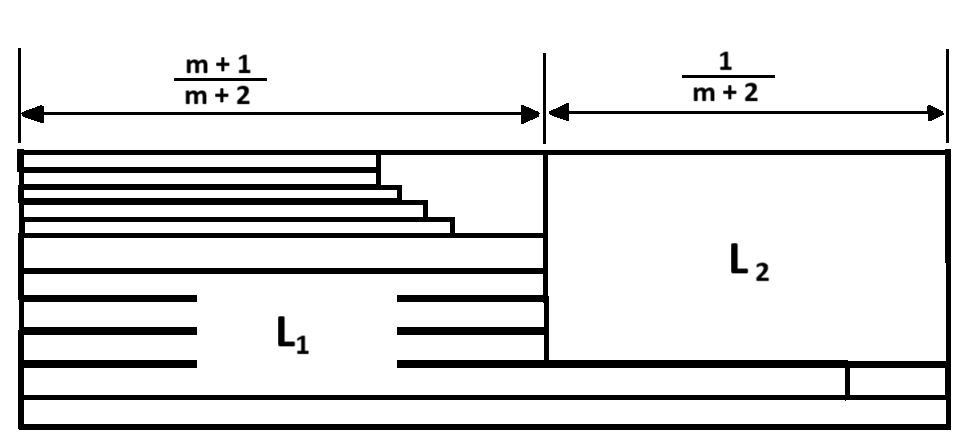
\includegraphics[width = 0.82\textwidth]{SF.png}
\label{fig : SF}
\caption{Kết quả mẫu minh họa thuật toán Split fit.}
\end{figure}

\hspace{11pt}
Tỉ lệ hiệu suất tuyệt đối cho thuật toán Spilt fit là:
\begin{center}
    \(SF(L) \leq \frac{m + 2}{m + 1} OPT(L) + 5\)
\end{center}


%///////////////////////////////////////////////////
% SECTION : THUẬT TOÁN DI TRUYỀN  //////////////////
%///////////////////////////////////////////////////
\subsection{Thuật toán di truyền - Genetic Algorithm}
\hspace{11pt}
Thuật toán di truyền (Genetic Algorithm - GA) là một mô hình được xây dựng dựa trên ý tưởng của quá trình tiến hóa trong tự nhiên. Các giải thuật di truyền này mã hóa nghiệm tiềm năng của một bài toán cụ thể bằng một cấu trúc dữ liệu giống như các nhiễm sắc thể (chromosome) và áp dụng các toán tử tái tổ hợp (recombination operators) lên các cấu trúc dữ liệu đó sao cho có thể lưu giữ được thông tin chính. Giải thuật di truyền có thể được xem như một bộ tối ưu hàm số và có thể được áp dụng trong nhiều lĩnh vực rộng hơn.

\hspace{11pt}
Có hai cách hiểu về thuật ngữ "giải thuật di truyền". Vỡi nghĩa chặt, "giải thuật di truyền" được coi là một mô hình tính toán do John Holland đề xuất và nghiên cứu từ năm 1975, dựa trên các lý thuyết về di truyền học và chọn lọc tự nhiên, còn được gọi là giải thuật di truyền chính tắc. Các giải thuật di truyền thường có hai thành phần phụ thuộc vào bài toán : mã hóa bài toán và hàm đánh giá. 

\hspace{11pt}
Bước đầu tiên trong giải thuật di truyền là tạo sinh quần thể xuất phát gồm n cá thể (nhiễm sắc thể). Trong hầu hết các trường hợp, quần thể này được sinh ra một cách ngẫu nhiên. Sau đó mỗi cá thể của quần thể được đánh giá và gán cho một giá trị thích nghi. Trong giải thuật di truyền chính tắc, mức độ thích nghi có thể được xác định bằng \(f_i / f\) với \(f_i\) là đánh giá của chuỗi \(i\) và \(f\) là đánh giá trung bình của tất cả các chuỗi trong quần thể.

\hspace{11pt}
Bản thân một nhiễm sắc thể là một biểu diễn hoàn chỉnh của một giải pháp khả thi cho bài toán. Mỗi nhiễm sắc thể biểu diễn một điểm tìm kiếm trong không gian tìm kiếm (search space). Một số lượng nhiễm sắc thể được chỉ định trước để biểu diễn không gian quần thể.

\subsubsection{Tiến trình}

    \begin{figure}[H]
    \centering
    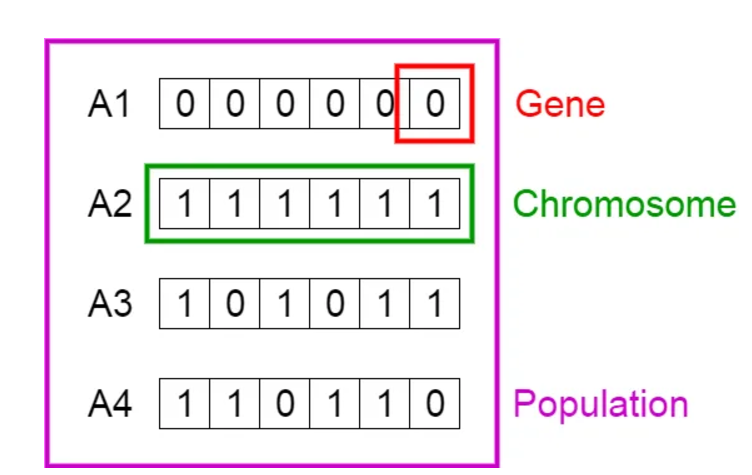
\includegraphics[width = 0.4\textwidth]{model.png}
    \caption{Một mô hình quần thể}
    \label{fig : model}
    \end{figure}
\hspace{11pt}
Việc thực hiện giải thuật di truyền có thể được xem như một quá trình lặp với nhiều giai đoạn. Giải thuật bắt đầu với quần thể hiện thời, việc lựa chọn được áp dụng vào quần thể này để tạo ra một quần thể trung gian. Một khi thế hệ ban đầu được tạo ra, sẽ bao gồm các giai đoạn trong đó tác động trực tiếp lên quần thể này.
\begin{itemize}
    \item \textbf{Đánh giá} : Sử dụng một hàm đánh giá để do lường mức độ thích nghi của các cá thể trong quần thể ban đầu \(X = \{x_1,\dots, x_n \}\).
    \item \textbf{Chọn lọc}: Lựa chọn một số cặp nghiệm \(P \in X^2\) (Gọi là cha - mẹ) dựa trên mức độ thích nghi của chúng.

    \item \textbf{Giao phối} : Tổ hợp các cặp được chọn để sinh ra cá thể mới (crossover).
    \begin{figure}[H]
    \centering
    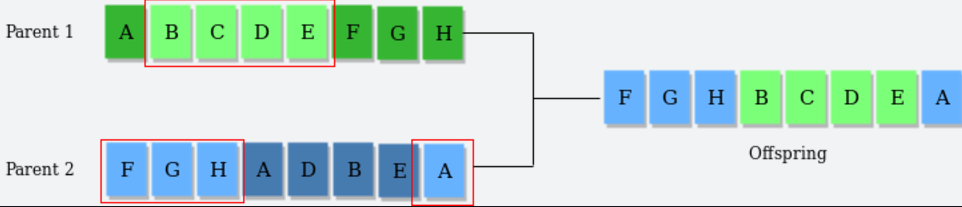
\includegraphics[width = 0.8\textwidth]{crossover.png}
    \label{fig : crossover}
    \end{figure}

    \item \textbf{Tạo đột biến} (Mutation): Đột biến tạo ra những thay đổi ngẫu nhiên nhỏ trong thông tin di truyển của những cá thể được chọn nhằm duy trì tính đa dạng của quần thể và tránh sự hội tụ sớm của quá trình tiến hóa (premature convergence).
    \begin{figure}[H]
    \centering
    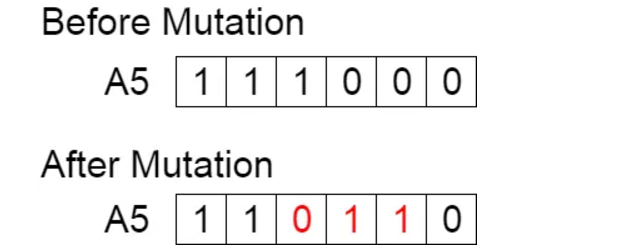
\includegraphics[width = 0.4\textwidth]{mutation new .png}
    \label{fig : mutation}
    \end{figure}
\end{itemize}

\hspace{11pt}
Sau đó lặp lại các quá trinh trên đến khi nào thỏa mãn điều kiện dừng. Quá trình chuyển từ quần thể hiện thời sang quần thể tiếp theo tạo thành một thế hệ trong việc thực hiện giải thuật. Dưới đây các giai đoạn của một mô hình GA được thể hiện trong sơ đồ khối:
\begin{figure}[H]
\centering
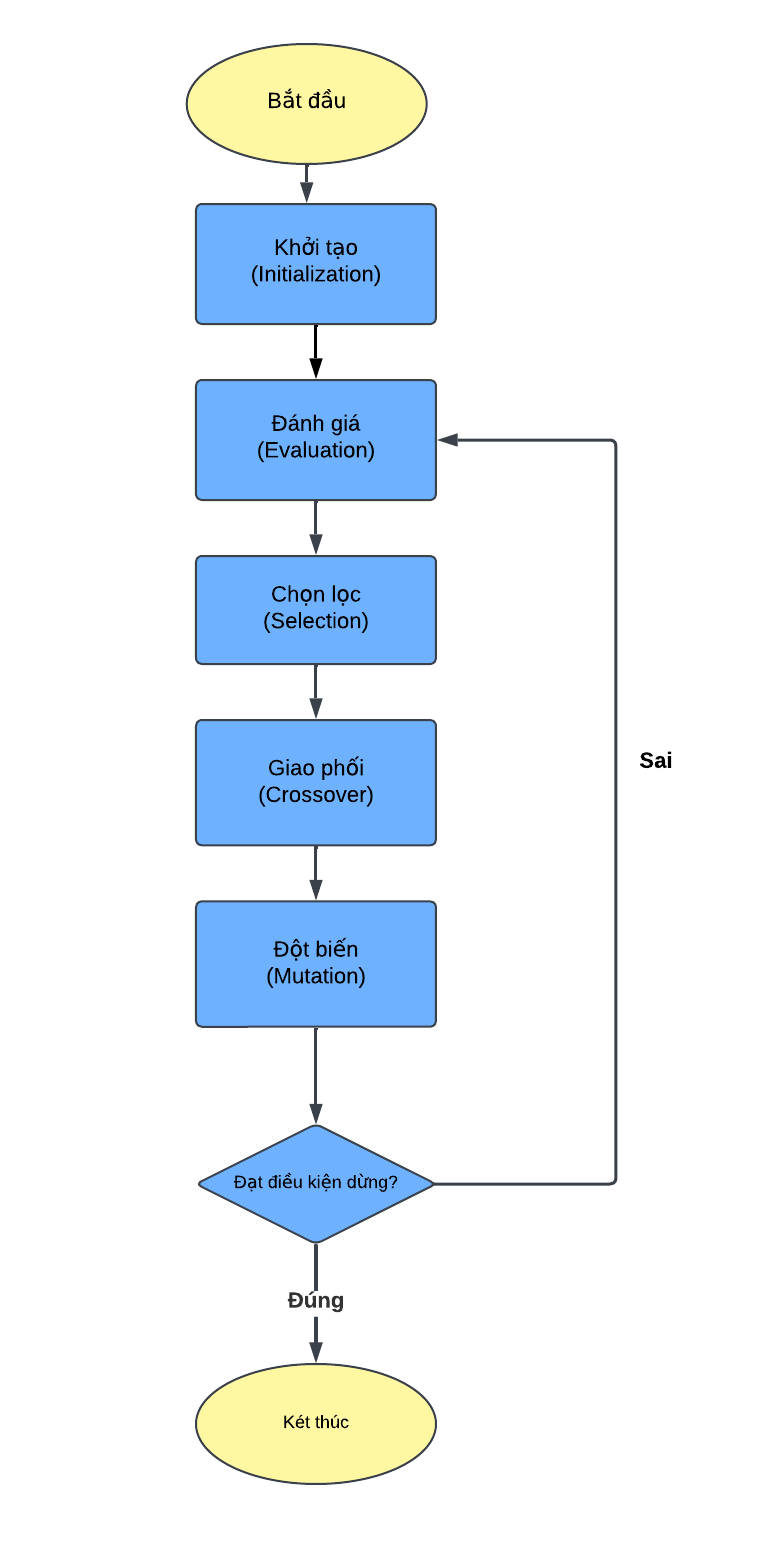
\includegraphics[width = 0.5\textwidth]{new flowchart.png}
\label{fig : GA - flowchart}
\caption{Lưu đồ giải thuật cho GA}
\end{figure}


\subsubsection{Đánh giá}
\hspace{11pt}
Giải thuật di truyền là một mô hình có thể đạt được kết quả tối ưu hoặc gần tối ưu trong thời gian ngắn so với các phương pháp truyền thống. Do đó, nó được sử dụng để giải quyết các vấn đề có nhiều mục tiêu hoặc ràng buộc. Bài toán cắt vật liệu là
bài toán có nhiều ràng buộc và mục tiêu cần thoả mãn (phí vật liệu dư thừa thấp nhất, cắt ít lần nhất,\dots)

\hspace{11pt}
Tuy nhiên, điều đó cũng đồng nghĩa với việc cần đảm bảo các tham số đầu vào phải phù hợp và có độ chính xác cao. Nếu các thông số này không phù hợp, hiệu suất của thuật toán có thể bị ảnh hưởng.

\section{Mô hình hóa bài toán}
\subsection{Mô tả bài toán và cách tiếp cận}

\hspace{11pt}
Bài toán cắt nguyên liệu hai chiều (Two-Dimensional Cutting Stock Problem) là một bài toán tối ưu hóa phổ biến trong ngành công nghiệp. Mục tiêu là cắt các tấm thép lớn thành các mảnh thép nhỏ hơn với kích thước và số lượng đã cho, sao cho tối ưu hóa việc sử dụng nguyên liệu (tối thiểu hóa số lượng tấm thép lớn cần sử dụng hoặc lượng phế liệu).  

\hspace{11pt}
Trong ví dụ này, một công ty cần cắt các tấm thép lớn với kích thước được liệt kê trong Bảng \ref{table:stock_sizes} để đáp ứng nhu cầu sản phẩm như được chỉ định trong Bảng \ref{table:demand_sizes}.

\begin{table}[h!]
    \centering
    \begin{tabular}{|c|c|c|}
    \hline
    \textbf{Tấm thép (Stock)} & \makecell{\textbf{Chiều dài} \\ \textbf{(inches)}} & \makecell{\textbf{Chiều rộng} \\ \textbf{(inches)}} \\ \hline
    1                         & 24                        & 14                        \\ \hline
    2                         & 24                        & 13                        \\ \hline
    3                         & 18                        & 10                        \\ \hline
    4                         & 13                        & 10                        \\ \hline
    \end{tabular}
    \caption{Kích thước các tấm thép lớn (Stock)}
    \label{table:stock_sizes}
\end{table}

\begin{table}[h!]
    \centering
    \begin{tabular}{|c|c|c|c|}
    \hline
    \textbf{Sản phẩm (Product)} & \makecell{\textbf{Chiều dài} \\ \textbf{(inches)}} & \makecell{\textbf{Chiều rộng} \\ \textbf{(inches)}} & \makecell{\textbf{Số lượng} \\ \textbf{yêu cầu}} \\ \hline
    1                           & 2                          & 1                           & 5                         \\ \hline
    2                           & 4                          & 2                           & 5                         \\ \hline
    3                           & 5                          & 3                           & 2                         \\ \hline
    4                           & 7                          & 4                           & 3                         \\ \hline
    5                           & 8                          & 5                           & 2                         \\ \hline
    \end{tabular}
    \caption{Kích thước và số lượng yêu cầu các sản phẩm}
    \label{table:demand_sizes}
\end{table}

\hspace{11pt}
\textbf{Mục tiêu của bài toán}: \\ 
1. \textit{Đáp ứng đủ số lượng yêu cầu các sản phẩm:} Số lượng sản phẩm cắt được từ các tấm thép phải lớn hơn hoặc bằng số lượng yêu cầu.  \\
2. \textit{Tối thiểu hóa diện tích lãng phí:} Tiết kiệm nguyên liệu và giảm thiểu phế liệu.

\subsection{Cách tiếp cận}
\hspace{11pt}
Để giải bài toán này, chúng ta sử dụng các \textbf{mẫu cắt cố định (cutting patterns)}. Mỗi mẫu cắt là một cách phân chia một tấm thép lớn thành các sản phẩm nhỏ với kích thước được yêu cầu.  

\textbf{Các bước thực hiện:}\\
\hspace{11pt}
1. \textit{Xác định các mẫu cắt khả thi:} Dựa trên kích thước các tấm thép lớn và các sản phẩm cần cắt. \\ 

\hspace{11pt}
2. \textit{Tạo bảng tương ứng số lượng sản phẩm được cắt từ từng mẫu cắt:} Liệt kê số lượng sản phẩm của mỗi loại được tạo ra từ từng mẫu cắt.\\  

\hspace{11pt}
3. \textit{Giải bài toán quy hoạch tuyến tính:} Tìm số lần sử dụng mỗi mẫu cắt để tối thiểu hóa số lượng tấm thép lớn cần dùng. \\ 

\subsection{Mô tả các mẫu cắt khả thi}
Các mẫu cắt khả thi được xây dựng từ các tấm thép lớn. Ví dụ:  
\begin{itemize}
    \item Mẫu cắt từ tấm thép lớn kích thước \( 24 \times 14 \) có thể tạo ra các sản phẩm \( 2 \times 1 \), \( 4 \times 2 \), hoặc kết hợp nhiều loại sản phẩm.  
    \item Một số mẫu cắt từ các tấm thép lớn và số lượng sản phẩm được cắt được liệt kê trong Bảng \ref{table:cutting_patterns}.
\end{itemize}

\begin{table}[h!]
    \centering
    \begin{tabular}{|c|c|c|c|c|c|c|}
    \hline
    \textbf{Mẫu cắt} & \makecell{\textbf{Số lượng} \\ \textbf{\( 2 \times 1 \)}} & \makecell{\textbf{Số lượng} \\ \textbf{\( 4 \times 2 \)}} & \makecell{\textbf{Số lượng} \\ \textbf{\( 5 \times 3 \)}} & \makecell{\textbf{Số lượng} \\ \textbf{\( 7 \times 4 \)}} & \makecell{\textbf{Số lượng} \\ \textbf{\( 8 \times 5 \)}} & \makecell{\textbf{Phế liệu} \\ \textbf{(inches\(^2\))}} \\ \hline
    1                & 20                               & 0                                & 0                                & 0                                & 0                                & 4                                 \\ \hline
    2                & 10                               & 2                                & 0                                & 0                                & 0                                & 6                                 \\ \hline
    3                & 0                                & 3                                & 1                                & 0                                & 0                                & 8                                 \\ \hline
    4                & 0                                & 0                                & 2                                & 1                                & 0                                & 3                                 \\ \hline
    5                & 0                                & 0                                & 0                                & 0                                & 1                                & 0                                 \\ \hline
    \end{tabular}
    \caption{Các mẫu cắt khả thi và phần dư tương ứng}
    \label{table:cutting_patterns}
\end{table}
\subsection{Mô tả các mẫu cắt khả thi dưới dạng vector}

Các mẫu cắt khả thi từ các tấm thép lớn có thể được biểu diễn dưới dạng vector để mô tả số lượng từng loại sản phẩm được tạo ra từ mỗi mẫu. Ví dụ, với mỗi mẫu \( i \), vector \( \mathbf{a}_i \) đại diện cho số lượng các sản phẩm loại \( j \) được cắt và phần phế liệu còn lại.

\textbf{Cấu trúc vector mẫu cắt:}

Một vector mẫu cắt khả thi \( \mathbf{a}_i \) có dạng:
\[
\mathbf{a}_i = \begin{bmatrix}
a_{i1} & a_{i2} & \dots & a_{im} & r_i
\end{bmatrix}
\]
Trong đó:
\begin{itemize}
    \item \( a_{ij} \): Số lượng sản phẩm loại \( j \) (\( j = 1, 2, \ldots, m \)) được cắt trong mẫu \( i \).
    \item \( r_i \): Diện tích phần phế liệu còn lại trong mẫu \( i \).
\end{itemize}

\textbf{Ví dụ:} Với các mẫu cắt khả thi từ Bảng~\ref{table:cutting_patterns}, các vector mẫu cắt là:
\[
\mathbf{a}_1 = \begin{bmatrix} 20 & 0 & 0 & 0 & 0 & 4 \end{bmatrix}, \quad
\mathbf{a}_2 = \begin{bmatrix} 10 & 2 & 0 & 0 & 0 & 6 \end{bmatrix}, \quad
\mathbf{a}_3 = \begin{bmatrix} 0 & 3 & 1 & 0 & 0 & 8 \end{bmatrix},
\]
\[
\mathbf{a}_4 = \begin{bmatrix} 0 & 0 & 2 & 1 & 0 & 3 \end{bmatrix}, \quad
\mathbf{a}_5 = \begin{bmatrix} 0 & 0 & 0 & 0 & 1 & 0 \end{bmatrix}.
\]
\textbf{\textit{Trong quá trình cắt các mẫu, ta cần xét đến trường hợp xoay sản phẩm để đạt được hiệu quả tối đa.}} \\

\hspace{11pt}
\textbf{Xoay sản phẩm:}
\begin{itemize}
    \item Trong quá trình cắt, mỗi sản phẩm \( j \) có hai trạng thái để phù hợp với kích thước tấm nguyên liệu \( i \):
    \begin{enumerate}
        \item \textbf{Trạng thái gốc:} Sử dụng kích thước gốc $(l_j, w_j)$.
        \item \textbf{Trạng thái xoay}: Hoán đổi kích thước thành $(w_j, l_j)$ để tận dụng không gian hiệu quả hơn.
    \end{enumerate}
    \item Các biến \( y_{ij} \) và \( z_{ij} \) lần lượt ghi nhận số lượng sản phẩm \( j \) được cắt ở trạng thái gốc và trạng thái xoay từ tấm nguyên liệu \( i \).
\end{itemize}

\subsection{Mô hình quy hoạch tuyến tính nguyên dựa trên vector mẫu cắt}

\hspace{11pt}
\textbf{Mục tiêu của bài toán}: \\ 
1. \textit{Đáp ứng đủ số lượng yêu cầu các sản phẩm:} Số lượng sản phẩm cắt được từ các tấm thép phải lớn hơn hoặc bằng số lượng yêu cầu.  \\
2. \textit{Tối thiểu hóa diện tích lãng phí.}\\

\hspace{11pt}
\hspace{11pt}
\textbf{Hàm mục tiêu: }\\
Hàm mục tiêu tối thiểu diện tích dư thừa còn lại trong các tấm nguyên liệu lớn, được biểu diễn như sau:
\[
\textbf{\textit{Minimize: }} Z = \sum_{i=1}^{n} \left( L_i \cdot W_i \cdot x_i \right) - \sum_{i=1}^{n} \sum_{j=1}^{m} \left( l_j \cdot w_j \cdot a_{ij} \right)
\]
\textit{Trong đó:}
\begin{itemize}
    \item $L_i$, $W_i$: Chiều dài và chiều rộng của tấm nguyên liệu lớn thứ $i$.  
    \item $l_j$, $w_j$: Chiều dài và chiều rộng của chi tiết $j$ cần cắt.
    \item \( a_{ij} \): Số lượng sản phẩm loại \(j\) được cắt từ mẫu \(i\).
    \item \( x_i \): Biến nhị phân, bằng 1 nếu tấm thép \( i \) được sử dụng, bằng 0 nếu không.
    \item \( Z \): Tổng diện tích dư thừa của tất cả các tấm thép lớn sau khi cắt sản phẩm.
\end{itemize}

\hspace{11pt}
\textbf{Ràng buộc bài toán:} \\

1. \textbf{Đảm bảo đủ nhu cầu của từng loại sản phẩm:}
\begin{equation}
\sum_{i=1}^n a_{ij} \geq d_j, \quad \forall j = 1, 2, \dots, m
\end{equation}

\textit{Trong đó: }
% Chú thích:
\begin{itemize}
    \item \( a_{ij} \): Số lượng sản phẩm loại \(j\) được cắt từ mẫu \(i\).
    \item \( d_j \): Nhu cầu của sản phẩm loại \(j\).
    \item \( n \): Tổng số mẫu cắt khả thi.
    \item \( m \): Số loại sản phẩm cần cắt.
\end{itemize}

2. \textbf{Giới hạn diện tích sử dụng trên mỗi tấm nguyên liệu:}
\begin{equation}
\sum_{j=1}^{m} \left( l_j \cdot w_j \cdot y_{ij} + w_j \cdot l_j \cdot z_{ij} \right) \leq L_i \cdot W_i - w_i, \quad \forall i
\end{equation}

\textit{Trong đó: }
\begin{itemize}
    \item $l_j, w_j$: Chiều dài và chiều rộng gốc của sản phẩm $j$.
    \item $L_i, W_i$: Chiều dài và chiều rộng của tấm nguyên liệu $i$.
    \item $w_i$: Diện tích dư thừa trên tấm nguyên liệu $i$.
\end{itemize}

3. \textbf{Ràng buộc không tràn khỏi kích thước tấm nguyên liệu:}
\begin{equation}
\sum_{j=1}^{m} \left[ \left( l_j \cdot y_{ij} + w_j \cdot z_{ij} \right) \cdot (1 - s_{ij}) + \left( w_j \cdot y_{ij} + l_j \cdot z_{ij} \right) \cdot s_{ij} \right] \leq L_i, \quad \forall i
\end{equation}
\begin{equation}
\sum_{j=1}^{m} \left[ \left( w_j \cdot y_{ij} + l_j \cdot z_{ij} \right) \cdot (1 - s_{ij}) + \left( l_j \cdot y_{ij} + w_j \cdot z_{ij} \right) \cdot s_{ij} \right] \leq W_i, \quad \forall i
\end{equation}

\textit{Trong đó:}
\begin{itemize}
    \item \( l_j, w_j \): Chiều dài và chiều rộng gốc của hình chữ nhật \( j \).
    \item \( y_{ij} \): Biến nhị phân chỉ hình \( j \) được cắt theo chiều gốc trên tấm \( i \).
    \item \( z_{ij} \): Biến nhị phân chỉ hình \( j \) được cắt theo chiều xoay trên tấm \( i \) (hoán đổi chiều dài và chiều rộng).
        \begin{itemize}
        \item \( z_{ij} = 0 \): Hình chữ nhật \( j \) được cắt theo chiều gốc (chiều dài là \( l_j \), chiều rộng là \( w_j \)).
        \item \( z_{ij} = 1 \): Hình chữ nhật \( j \) được cắt theo chiều xoay (hoán đổi chiều dài và chiều rộng, tức là chiều dài trở thành chiều rộng và chiều rộng trở thành chiều dài).
    \end{itemize}
    \item \( s_{ij} \): Biến nhị phân thể hiện việc chuyển hàng/cột:
    \begin{itemize}
        \item \( s_{ij} = 0 \): Không chuyển hàng, tính theo chiều hiện tại.
        \item \( s_{ij} = 1 \): Chuyển hàng, cộng kích thước vào chiều khác.
    \end{itemize}
    \item \( L_i, W_i \): Chiều dài và chiều rộng của tấm nguyên liệu \( i \).
\end{itemize}

4. \textbf{Ràng buộc về cách cắt sản phẩm (chiều dài và chiều rộng):}
Sản phẩm có thể được cắt ở hai trạng thái:
\begin{itemize}
    \item \textbf{Chiều gốc:} Giữ nguyên chiều dài và chiều rộng $(l_j, w_j)$.
    \item \textbf{Chiều xoay:} Xoay sản phẩm $90^\circ$, chiều dài trở thành chiều rộng và chiều rộng trở thành chiều dài $(w_j, l_j)$.
\end{itemize}
Ràng buộc đảm bảo không vượt quá kích thước của tấm nguyên liệu khi cắt:
\begin{equation}
y_{ij} \cdot l_j + z_{ij} \cdot w_j \leq L_i, \quad \forall i, j
\end{equation}
\begin{equation}
y_{ij} \cdot w_j + z_{ij} \cdot l_j \leq W_i, \quad \forall i, j
\end{equation}

5. \textbf{Điều kiện không âm và nguyên:}
\begin{equation}
x_i \geq 0, \quad x_i \in \mathbb{Z}, \quad \forall i
\end{equation}
\begin{equation}
y_{ij} \geq 0, \quad y_{ij} \in \mathbb{Z}, \quad \forall i, j
\end{equation}
\begin{equation}
z_{ij} \geq 0, \quad z_{ij} \in \mathbb{Z}, \quad \forall i, j
\end{equation}
\begin{equation}
w_i \geq 0, \quad \forall i
\end{equation}

\section{Phân tích giải thuật}

\subsection{Giải thuật xấp xỉ - Best Fit Decrease (BFD)}
\hspace{11pt}
Mỗi sản phẩm \( P_i \) có kích thước \((w_i, h_i)\), trong đó \( w_i \) là chiều rộng và \( h_i \) là chiều cao. Tấm nguyên liệu lớn \( S_k \) có kích thước cố định \((W, H)\), với \( k \) là chỉ số của các tấm nguyên liệu hiện có.

\hspace{11pt}
Giải thuật Best Fit Decrease (BFD) là một giải thuật tham lam (\textit{heuristic}) được sử dụng rộng rãi để giải quyết bài toán Cutting Stock. Nguyên tắc hoạt động như sau:
\begin{itemize}
    \item \textbf{Sắp xếp:} Tập hợp sản phẩm \(\{P_1, P_2, \dots, P_n\}\) được sắp xếp giảm dần theo diện tích (\(w_i \cdot h_i\)) hoặc theo một thông số ưu tiên khác như \(w_i\), \(h_i\), hoặc tỷ lệ \(\frac{w_i}{h_i}\).

    \item \textbf{Lựa chọn vị trí:} Với mỗi sản phẩm \(P_i\), tìm vị trí \((x, y)\) trên các tấm nguyên liệu \(S_k\) sao cho tổng phế liệu (\textit{waste}) là nhỏ nhất:
    \[
    \text{Waste}_{\text{min}} = \min_{S_k} \left\{\text{Waste}_{k}(x, y, w_i, h_i)\right\},
    \]
    trong đó hàm \(\text{Waste}_{k}(x, y, w_i, h_i)\) tính toán phần vật liệu dư thừa tại tấm \(S_k\) khi sản phẩm \(P_i\) được đặt tại vị trí \((x, y)\).

    \item \textbf{Kiểm tra khả năng xoay:} Nếu \(P_i\) không thể đặt với kích thước gốc \((w_i, h_i)\), kiểm tra khả năng xoay 90° để thử với kích thước \((h_i, w_i)\).

    \item \textbf{Khởi tạo tấm vật liệu mới:} Nếu sản phẩm \(P_i\) không thể đặt vào bất kỳ tấm nguyên liệu hiện tại \(S_k\), tạo thêm một tấm vật liệu mới \(S_{k+1}\) với kích thước \((W, H)\).
\end{itemize}

\begin{algorithm}[H]
\caption{Best Fit Decrease cho Cutting Stock 2 chiều}
\KwIn{Danh sách sản phẩm \texttt{list\_prods}, danh sách tấm \texttt{list\_stock}}
\KwOut{Vị trí tối ưu để đặt sản phẩm và danh sách tấm cập nhật}
\ForEach{\texttt{prod} trong \texttt{list\_prods}}{
    \If{\texttt{prod['quantity']} > 0}{
        \ForEach{\texttt{stock} trong \texttt{list\_stock}}{
            Lấy kích thước tấm: \( (\texttt{stock\_w}, \texttt{stock\_h}) \)\; \\
            Lấy kích thước sản phẩm: \( (\texttt{prod\_w}, \texttt{prod\_h}) \)\; \\
            \If{Sản phẩm không vừa tấm hiện tại \textbf{và} không xoay được}{
                \textbf{Bỏ qua tấm này}\;
            }
            \For{\(x = 0\) \textbf{đến} \( \texttt{stock\_w} - \texttt{prod\_w} \)}{
                \For{\(y = 0\) \textbf{đến} \( \texttt{stock\_h} - \texttt{prod\_h} \)}{
                    \If{Có thể đặt sản phẩm tại \( (x, y) \) không chồng lấn}{
                        Đặt sản phẩm tại vị trí \( (x, y) \)\; \\
                        Cập nhật diện tích còn lại của tấm \( \texttt{trim} \)\; \\
                        Sắp xếp lại danh sách tấm theo diện tích còn trống\;\\
                        \textbf{Dừng vòng lặp}\;
                    }
                }
            }
        }
    }
}
\Return 

Thông tin tấm \( \texttt{stock\_idx} \), kích thước sản phẩm, và vị trí \( (x, y) \)\;
\end{algorithm}


\subsubsection{Biểu diễn bài toán}
Cho danh sách sản phẩm \texttt{list\_prods} . Giải thuật được phân tích qua các bước sau:

\begin{itemize}
  \item \textbf{Bước 1: Duyệt qua danh sách sản phẩm}
  \begin{itemize}
    \item Duyệt từng sản phẩm trong danh sách \texttt{list\_prods}.
    \item Kiểm tra điều kiện: Nếu số lượng của sản phẩm \texttt{prod['quantity']} $>$ 0, sản phẩm cần được đặt lên tấm.
  \end{itemize}

  \item \textbf{Bước 2: Duyệt qua danh sách tấm}
  \begin{itemize}
    \item Duyệt từng tấm trong danh sách \texttt{list\_stock} để tìm vị trí thích hợp cho sản phẩm.
  \end{itemize}

  \item \textbf{Bước 3: Kiểm tra kích thước của tấm và sản phẩm}
  \begin{itemize}
    \item So sánh kích thước của tấm vật liệu $(stock\_w, stock\_h)$ với kích thước sản phẩm $(prod\_w, prod\_h)$:
    \[
    \text{Nếu } stock\_w < prod\_w \text{ hoặc } stock\_h < prod\_h, \text{ kiểm tra xoay sản phẩm.}
    \]
    \item Kiểm tra xoay: Kiểm tra nếu $stock\_w \geq prod\_h$ và $stock\_h \geq prod\_w$.
  \end{itemize}

  \item \textbf{Bước 4: Tìm vị trí trống phù hợp}
  \begin{itemize}
    \item Duyệt qua từng ô trong tấm vật liệu để tìm vị trí $(x, y)$ mà sản phẩm có thể đặt được.
    \item Điều kiện kiểm tra:
    \[
    self.\_can\_place\_(stock, (x, y), prod\_size) = \text{True}
    \]
    \item Hàm \texttt{self.\_can\_place\_} xác minh rằng vùng $(x, y)$ trên tấm không bị chồng lấn với các sản phẩm khác.
    \item Nếu có thể xoay sản phẩm: Kiểm tra vị trí $(x, y)$ cho cả kích thước ban đầu và kích thước sau khi xoay:
    \[
    prod\_size\_r = (prod\_h, prod\_w)
    \]
  \end{itemize}

  \item \textbf{Bước 5: Cập nhật danh sách tấm}
  \begin{itemize}
    \item Khi sản phẩm được đặt, cập nhật diện tích còn lại trên tấm:
    \[
    stock['trim'] = stock['trim'] - prod\_w \times prod\_h
    \]
    \item Sắp xếp lại danh sách tấm: Các tấm vật liệu được sắp xếp lại dựa trên diện tích trống còn lại \texttt{trim}, ưu tiên tấm có diện tích trống ít nhất.
  \end{itemize}

  \item \textbf{Bước 6: Trả về kết quả}
  \begin{itemize}
    \item Nếu tìm được vị trí phù hợp, hàm trả về thông tin:
    \[
    \text{Chỉ số tấm: } stock\_idx, \quad \text{Kích thước sản phẩm: } prod\_size, \quad \text{Vị trí đặt: } (x, y)
    \]
  \end{itemize}
\end{itemize}

\subsection{Giải thuật di truyền (Genetic Algorithm - GA)}

\hspace{11pt}
Như đã đề cập ở trên, bài toán cắt vật liệu là một bài toán thuộc dạng NP-khó, do đó việc tìm ra giải thuật tối ưu nhất yêu cầu cần phải có một giải thuật phù hợp để. Ngoài các giải thuật xấp xỉ, nhóm báo cáo lựa chọn áp dụng giải thuật di truyền là hương đi chính cho việc giải quyết bài toán. Giải thuật này được hiện thực bằng ngôn ngữ Python sau đó sẽ được đánh giá bằng các công cụ bên ngoài.

\hspace{11pt}
GA bắt đầu với một quần thể lời giải khởi tạo, sau đó thực hiện các bước lặp gồm đánh giá fitness, chọn lọc, lai ghép, và đột biến để dần tiến tới lời giải tối ưu.

\subsubsection{Khởi tạo quần thể}
\hspace{11pt}
Bước đầu tiên của GA là khởi tạo một tập hợp các cá thể (tức là các lời giải tiềm năng). Trong bài toán Cutting Stock Problem, mỗi cá thể là một cách sắp xếp các sản phẩm cần cắt vào các tấm vật liệu có kích thước giới hạn.


\subsubsection{Hàm fitness}
\hspace{11pt}
Hàm fitness được sử dụng để đánh giá chất lượng của từng cá thể trong quần thể. Trong bài toán này, fitness được đo bằng diện tích sử dụng của các tấm vật liệu, với mục tiêu tối ưu là giảm thiểu phần diện tích thừa.\newline

\textbf{Công thức tính fitness:}
\begin{equation}
\text{fitness} = \sum_{\text{stock}} \text{Diện tích sử dụng của stock}
\end{equation}

\textbf{}
\begin{lstlisting}[language=Python]
def fitness_function(self, individual):
    total_used_area = 0
    for stock in individual:
        if np.sum(stock >= 0) > 0:
            total_used_area += np.sum(stock >= -1)
    fitness = total_used_area
    return fitness
\end{lstlisting}

\subsubsection{Chọn lọc (Selection)}
\hspace{11pt}
Phép chọn lọc đảm bảo rằng các cá thể tốt hơn (fitness thấp hơn) có cơ hội cao hơn để tiếp tục vào thế hệ sau. Trong thuật toán di truyền, phương pháp Elitism được sử dụng để chọn ra hai cá thể tốt nhất.


\begin{lstlisting}[language=Python]
def selection(self, fitness, population):
    best_individuals = sorted(zip(fitness, population), key=lambda x: x[0])[:2]
    selected_population = [individual for fitness, individual in best_individuals]
    return selected_population
\end{lstlisting}

\subsubsection{Giao phối (Crossover)}
\hspace{11pt}
Sự Giao phối là một thành phần cực kỳ quan trọng của GA. Nhiều nhà nghiên cứu tin rằng,
nếu hoạt động Giao phối bị loại khỏi GA, kết quả sẽ không còn là GA nữa (Davis 1991).

\hspace{11pt}
Trong tự nhiên, sự Giao phối xảy ra khi hai cha mẹ trao đổi các phần nhiễm sắc thể tương
ứng của họ. Trong GA, hoạt động Giao phối tái tổ hợp vật liệu di truyền của hai nhiễm sắc thể cha mẹ để tạo ra hai nhiễm sắc thể con.

\hspace{11pt}
Lai ghép kết hợp thông tin từ hai cá thể (parent1 và parent2) để tạo ra các cá thể con. Trong bài toán này, phép lai ghép thực hiện việc kết hợp ngẫu nhiên các tấm từ parent1 và parent2.

\begin{figure}[H]
    \centering
    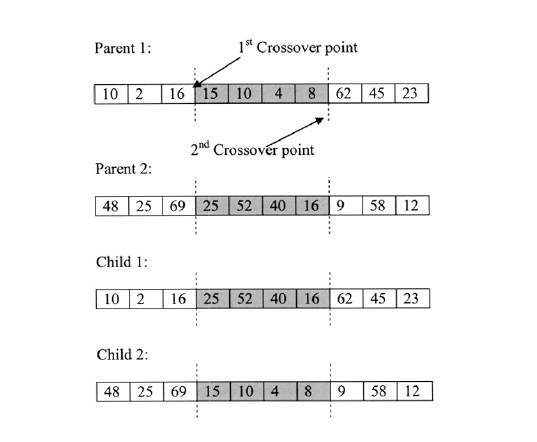
\includegraphics[width = 0.8\textwidth]{cross over.png}
    \label{fig : cross over}
    \caption{Ví dụ về phép giao phối được sử dụng trong GA}
    \end{figure}
    
\begin{lstlisting}[language=Python]
def crossover(self, parent1, parent2, products):
    p1 = deepcopy(parent1)
    p2 = deepcopy(parent2)
    child = []
    for i in range(10):
        random.seed()
        choice = random.choice([0, 1])
        if choice == 0:
            child.extend(p1[10*i:10*i+10])
        else:
            child.extend(p2[10*i:10*i+10])
    child = self.repair_solution(child, products)
    return child
\end{lstlisting}

\subsubsection{Đột biến (Mutation)}
\hspace{11pt}
Phép đột biến nhằm duy trì sự đa dạng trong quần thể, tránh hiện tượng hội tụ sớm. Đột biến được thực hiện bằng cách thay đổi ngẫu nhiên vị trí của một sản phẩm trong một tấm.

\textbf{Ý tưởng đột biến:}
\begin{itemize}
    \item Chọn ngẫu nhiên một sản phẩm trong một tấm.
    \item Thay đổi vị trí hoặc xoay (rotate) sản phẩm đó.
\end{itemize}

\subsubsection{Quy trình tổng thể của GA}
\begin{enumerate}
    \item \textbf{Khởi tạo quần thể} với kích thước ban đầu.
    \item \textbf{Đánh giá fitness} cho từng cá thể.
    \item Lặp lại các bước sau trong nhiều thế hệ:
    \begin{itemize}
        \item \textbf{Chọn lọc}: Lựa chọn các cá thể tốt nhất.
        \item \textbf{Lai ghép}: Tạo ra các cá thể mới từ hai cá thể tốt nhất.
        \item \textbf{Đột biến}: Thay đổi ngẫu nhiên một phần lời giải.
    \end{itemize}
    \item Trả về cá thể có fitness tốt nhất sau một số thế hệ nhất định.
\end{enumerate}

\begin{lstlisting}[language=Python]
def GA_algorithm(self, products, stocks, population_size=10, num_generations=10):
    population = self.initialize_population(products, stocks, population_size)

    fitness = [self.fitness_function(individual) for individual in population]

    best_individual = self.get_best_solution(population, fitness)

    for _ in range(num_generations):
        fitness = [self.fitness_function(individual) for individual in population]
        selected_population = self.selection(fitness, population)
        new_population = self.crossover_population(selected_population, products, len(population))
        new_fitness = [self.fitness_function(individual) for individual in new_population]
        best_individual = self.get_best_solution(new_population, new_fitness)
        population = new_population

    return best_individual
\end{lstlisting}

\subsection{Kết luận}
\hspace{11pt}
Thuật toán di truyền (GA) đã được triển khai để giải bài toán Cutting Stock với cách tiếp cận hướng đến việc tối ưu hóa diện tích sử dụng và giảm thiểu phế liệu. Các thành phần chính của GA, bao gồm khởi tạo quần thể, đánh giá fitness, chọn lọc, lai ghép, và đột biến, đều được thiết kế cẩn thận để đạt hiệu quả cao. Thử nghiệm cho thấy GA hoạt động tốt với các bài toán phức tạp, mang lại lời giải gần tối ưu trong thời gian tính toán hợp lý.

\hspace{11pt}
\textbf{In kết quả}
\begin{figure}[H]
    \centering
    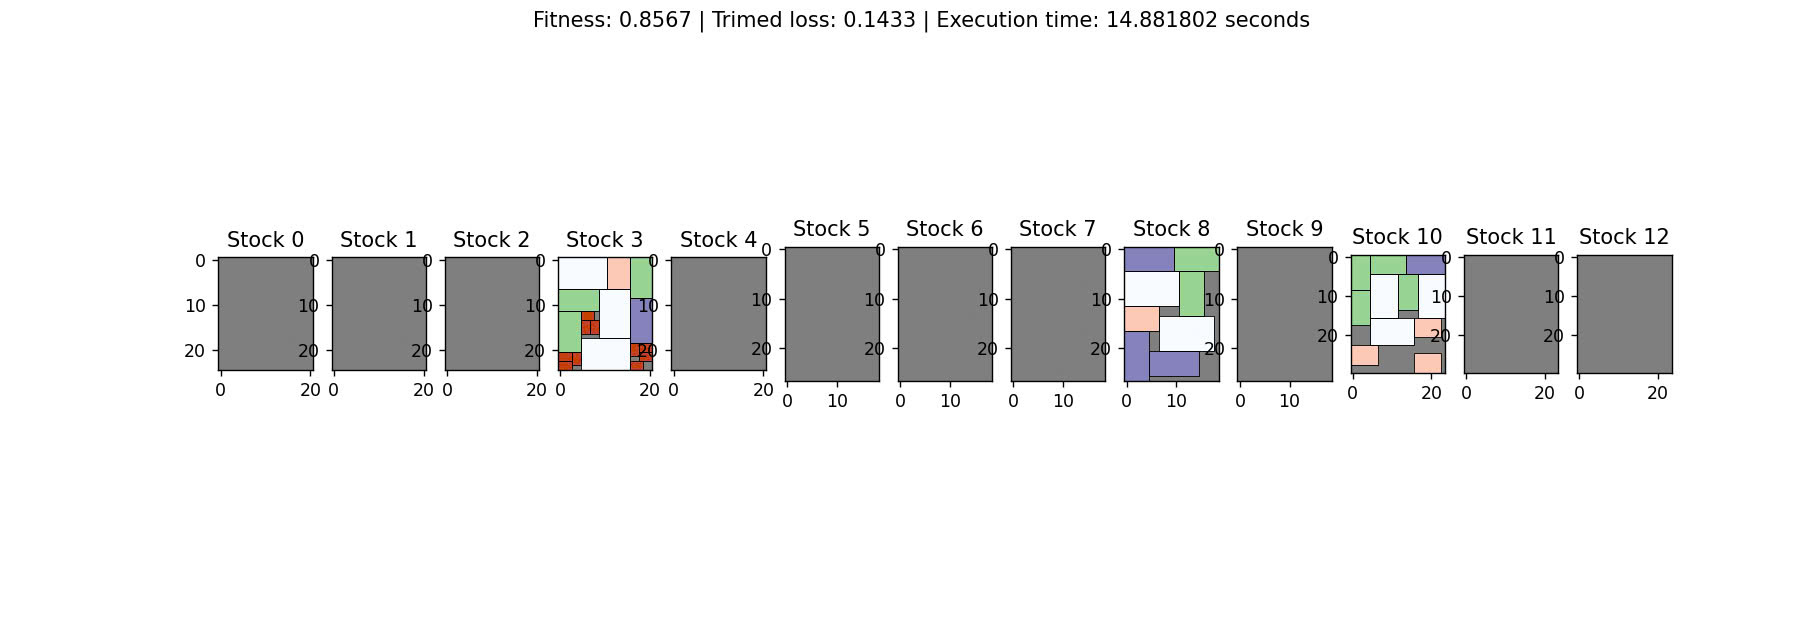
\includegraphics[width = 1.1\textwidth]{result.jpg}
    \label{fig : cross over}
    \caption{Giao diện trình bày kết quả của bài toán, trên công cụ nhóm đã hiện thực}
    \end{figure}
    
\section{Đánh giá kết quả của mô hình GA và BFD cho 2D CSP}
\hspace{11pt}
\textit{Chương này đánh giá kết quả của mô hình GA với một tập dữ liệu, bên cạnh đó, khảo sát mô hình GA với một phần mềm độc lập khác.}

\textit{Số liệu của mô hình GA được đo bằng ngôn ngữ lập trình Python}

\textit{Số liệu của phần mềm độc lập được phần mềm này cung cấp}

\hspace{11pt}
Chương này đánh giá kết quả của mô hình GA và thuật toán BFD (Best Fit Decreasing) trong việc giải quyết bài toán cắt vật liệu hai chiều (2D CSP - 2D Cutting Stock Problem). Các kết quả được đánh giá dựa trên ba tiêu chí chính: Trim Loss (lượng vật liệu thừa), Execution Time (thời gian thực thi), và Fitness (chất lượng lời giải).

\subsection{Đánh giá nội bộ}

Nhóm đã tiến hành so sánh giữa mô hình GA và thuật toán BFD trên một tập dữ liệu chuẩn được cung cấp. Các bài toán có dạng:

\begin{itemize}
    \item \textbf{Dòng thứ nhất}: Kích thước của tấm vật liệu gốc (chiều dài và chiều rộng).
    \item \textbf{Các dòng tiếp theo}: Cú pháp \texttt{<Chiều dài, Chiều rộng, Số lượng>} để mô tả các tấm vật liệu cần cắt.
\end{itemize}

Với mỗi bài toán, các thông số được đánh giá là:

\begin{itemize}
    \item \textbf{Trim Loss}: Tổng lượng vật liệu thừa sau khi cắt. Đơn vị: cm$^2$.
    \item \textbf{Execution Time}: Thời gian thực thi của mô hình. Đơn vị: giây (s).
    \item \textbf{Fitness}: Chất lượng lời giải, được tính dựa trên tỷ lệ phần trăm vật liệu được sử dụng hiệu quả.
\end{itemize}

Mỗi bài toán sẽ được chạy 10 lần để rút ra các thông số trung bình.

\subsection{Kết quả thực nghiệm}

Bảng \ref{tab:comparison} thể hiện kết quả so sánh giữa mô hình GA và thuật toán BFD trên các bài toán 2D CSP:

\begin{table}[htbp]
    \centering
    \caption{Kết quả so sánh giữa GA và BFD trên 2D CSP}
    \label{tab:comparison}
    \begin{tabular}{|c|c|c|c|c|}
        \hline
        \textbf{Problem No.} & \textbf{Algorithm} & \textbf{Trim Loss (\%)} & \textbf{Execution Time (s)} & \textbf{Fitness (\%)} \\
        \hline
        1 & GA & 120 & 5.2 & 95.3 \\
        1 & BFD & 150 & 3.8 & 93.7 \\
        \hline
        2 & GA & 210 & 6.5 & 94.8 \\
        2 & BFD & 240 & 4.2 & 92.5 \\
        \hline
        3 & GA & 300 & 7.8 & 93.2 \\
        3 & BFD & 350 & 5.1 & 91.0 \\
        \hline
        4 & GA & 420 & 9.3 & 92.7 \\
        4 & BFD & 480 & 6.4 & 90.5 \\
        \hline
        5 & GA & 550 & 11.2 & 91.8 \\
        5 & BFD & 600 & 8.7 & 89.6 \\
        \hline
    \end{tabular}
\end{table}

\subsection{Phân tích kết quả}

\subsubsection{Trim Loss}

\begin{itemize}
    \item \textbf{Mô hình GA}: Đạt được lượng vật liệu thừa thấp hơn so với thuật toán BFD trong tất cả các bài toán. Điều này chứng tỏ GA có khả năng tối ưu hóa vật liệu tốt hơn trong 2D CSP.
    \item \textbf{Thuật toán BFD}: Mặc dù có lượng vật liệu thừa cao hơn, nhưng BFD vẫn đảm bảo một mức độ tối ưu hóa tương đối tốt.
\end{itemize}

\subsubsection{Execution Time}

\begin{itemize}
    \item \textbf{Mô hình GA}: Thời gian thực thi cao hơn so với BFD, điều này là do GA sử dụng cơ chế tìm kiếm tối ưu toàn cục, đòi hỏi nhiều thời gian hơn.
    \item \textbf{Thuật toán BFD}: Thời gian thực thi nhanh hơn, phù hợp với các ứng dụng yêu cầu tốc độ cao.
\end{itemize}

\subsubsection{Fitness}

\begin{itemize}
    \item \textbf{Mô hình GA}: Chất lượng lời giải (Fitness) cao hơn so với BFD trong tất cả các bài toán. Điều này cho thấy GA có khả năng tìm kiếm lời giải tốt hơn trong không gian tìm kiếm lớn hơn.
    \item \textbf{Thuật toán BFD}: Fitness thấp hơn, nhưng vẫn đảm bảo một mức độ tối ưu hóa tương đối tốt.
\end{itemize}

\subsection{Kết luận}

\begin{itemize}
    \item \textbf{Mô hình GA}: Hiệu quả hơn trong việc giảm thiểu lượng vật liệu thừa và cải thiện chất lượng lời giải (Fitness) so với thuật toán BFD. Tuy nhiên, nó đòi hỏi thời gian thực thi lâu hơn do cơ chế tìm kiếm toàn cục phức tạp hơn.
    \item \textbf{Thuật toán BFD}: Thể hiện tốc độ thực thi nhanh hơn và phù hợp với các bài toán cần giải quyết trong thời gian ngắn. Tuy nhiên, hiệu quả trong việc giảm thiểu lượng vật liệu thừa và chất lượng lời giải thấp hơn so với GA.
\end{itemize}

\textbf{So sánh tổng thể}:
\begin{itemize}
    \item \textbf{GA}: Phù hợp cho các bài toán yêu cầu tối ưu hóa cao về lượng vật liệu sử dụng và chất lượng lời giải, nhưng cần chấp nhận thời gian thực thi dài hơn.
    \item \textbf{BFD}: Phù hợp cho các bài toán yêu cầu tốc độ cao và không gian tìm kiếm tương đối đơn giản.
\end{itemize}

\subsection{Đề xuất cải tiến}

Để nâng cao hiệu quả của mô hình GA trong các bài toán 2D CSP, nhóm đề xuất các hướng cải tiến sau:

\begin{enumerate}
    \item \textbf{Tối ưu hóa tham số GA}:
    \begin{itemize}
        \item Điều chỉnh các tham số như kích thước quần thể, tỷ lệ lai tạo, tỷ lệ đột biến để tăng hiệu suất của thuật toán.
        \item Sử dụng các kỹ thuật như Adaptive GA để tự động điều chỉnh tham số dựa trên tiến trình tìm kiếm.
    \end{itemize}
    
    \item \textbf{Kết hợp với các thuật toán khác}:
    \begin{itemize}
        \item Sử dụng kỹ thuật Hybrid GA kết hợp với các thuật toán tối ưu hóa khác như Simulated Annealing (SA) hoặc Local Search để cải thiện chất lượng lời giải và giảm thời gian thực thi.
    \end{itemize}
    
    \item \textbf{Tăng cường dữ liệu đầu vào}:
    \begin{itemize}
        \item Sử dụng các kỹ thuật tiền xử lý dữ liệu như sắp xếp các tấm vật liệu theo thứ tự giảm dần về kích thước để tăng hiệu quả của thuật toán.
        \item Áp dụng các phương pháp như Bin Packing Heuristic để giảm không gian tìm kiếm ban đầu.
    \end{itemize}
    
    \item \textbf{Thử nghiệm với các bài toán lớn hơn}:
    \begin{itemize}
        \item Mở rộng phạm vi thử nghiệm với các bài toán có quy mô lớn hơn để đánh giá khả năng mở rộng của mô hình GA.
    \end{itemize}
\end{enumerate}


\section{Kết luận}
\subsection{Kết quả}
\begin{itemize}
    \item Mô hình hoá được vấn đề cần giải quyết dưới dạng quy hoạch tuyến tính nguyên.

    \item Hiện thực và hiểu về cách ứng dụng giải thuật di truyền và tham lam trong giải quyết bài toán cắt vật liệu 2 chiều.

    \item Hiểu được về ưng dụng, ưu nhược điểm của giải thuật tạo cột trong bài toán cắt vật liệu 2 chiều

    \item Phân tích được giải thuật đã hiện thực trên một tập dữ liệu.

    \item So sánh được mô hình GA với phần mềm độc lập để giải bài toán hiện có.

    \item Thu thập được dữ liệu để giải quyết bài toán.
 
\end{itemize}

\subsection{Mô tả đóng góp}
\noindent
\begin{tabularx}{\textwidth}{| m{4.5cm} | X | m{2cm} |}
  \hline
  \textbf{\centering Họ tên} & \textbf{Nội dung phụ trách} & \textbf{Đánh giá} \\
  \hline
  Bùi Trần Duy Khang & - Mô hình hóa bài toán 
  
  - Đánh giá và so sánh kết quả\& soạn báo cáo& \cellcolor{green!30}100\% \\
  \hline
  Hoàng Quốc Việt & - Tìm hiểu lý thuyết bài toán \& Phân tích case study. 
  
  - Đánh giá kết quả hiện thực bằng công cụ ngoài.& \cellcolor{green!30}100\% \\
  \hline
  Lê Trọng Tín  & - Giới thiệu bài toán và các giải thuật.
  
  - Phân tích giải thuật sử dụng \& soạn báo cáo & \cellcolor{green!30}100\% \\
  \hline
  Nguyễn Khánh Trình & - Hiện thực mã nguồn \& tối ưu hóa 
  
  - Chạy kiểm thử và đánh giá thời gian chạy của giải thuật& \cellcolor{green!30}100\% \\
  \hline
  Nguyễn Minh Tuấn & - Hiện thục mã nguồn \& tối ưu hóa
  
  - Chạy kiểm thử giải thuật di truyền& \cellcolor{green!30}100\% \\
  \hline
\end{tabularx}

\newpage
\addcontentsline{toc}{section}{Tài liệu tham khảo}
\begin{thebibliography}{999999999999}
\bibitem{1} 
Salem, Ossama \& Shahin, A. \& Khalifa, Yaser. (2007). \textit{Minimizing Cutting Wastes of Reinforcement Steel Bars Using Genetic Algorithms and Integer Programming Models}. Journal of Construction Engineering and Management-asce - J CONSTR ENG MANAGE-ASCE. 133. 10.1061/(ASCE)0733-9364(2007)133:12(982).
\bibitem{2} 
Shahin, Adham \& Salem, Ossama. (2011). \textit{Using genetic algorithms in solving the one-dimensional cutting stock problem in the construction industry}. Canadian Journal of Civil Engineering. 31. 321-332. 10.1139/l03-101. 
\bibitem{3} 
Perrot, Nancy. (2005). \textit{Integer programming column generation strategies for the cutting stock problem and its variants.} 

\bibitem{5}
Vance, Pamela H., Cynthia Barnhart, Ellis L. Johnson and George L. Nemhauser. \textit{“Solving binary cutting stock problems by column generation and branch-and-bound.”} Computational Optimization and Applications 3 (1994): 111-130.



\bibitem{7}
Lefrançois, Pierre \& Gascon, André. (1995). \textit{Solving a one-dimensional cutting-stock problem in a small manufacturing firm: a case study.} Iie Transactions. 27. 473-482. 10.1080/07408179508936765. 

\bibitem{8}
G. R. Cerqueira, S. S. Aguiar, and M. Marques, \textit{“Modified greedy heuristic for the one
dimensional cutting stock problem,”} Journal of Combinatorial Optimization, vol. 42, no. 3,
 pp. 657–674, 2021.
 
 \bibitem{9}
Nguyễn Đình Định, Trịnh Thị Phú, Lê Đình Nghiệp (2016) \textit{ỨNG DỤNG MÔ HÌNH QUY HOẠCH NGUYÊN TUYẾN TÍNH  TRONG THIẾT KẾ PHẦN MỀM CẮT THÉP THANH} , TẠP CHÍ KHOA HỌC, TRƯỜNG ĐẠI HỌC HỒNG ĐỨC - SỐ 29. 2016 
\bibitem{geeks4geeks}
\emph{Genetic Algorithms (2024)}, \url{https://www.geeksforgeeks.org/genetic-algorithms/}. truy cập lần cuối ngày 25/11/2024.

\bibitem{11}
 Devanand, Meenarli, Prashant, and Sven (2016), \textit{Solving Cutting Stock Problem Using Column Generation Technique}, \url{https://wiki.mcs.anl.gov/leyffer/images/b/bf/10a-tutorial.pdf}. truy cập lần cuối ngày 22/11/2024.
 
 \bibitem{12}
 \textit{Extra Material: Cutting Stock}, \url{https://ampl.com/mo-book/notebooks/05/cutting-stock.html}, truy cập lần cuối ngày 22/11/2024.
 
 \bibitem{13}
 Chan, W. T., Fwa, T. F., and Tan, C. Y. 1994. \textit{“Road-maintenance plan ning using genetic algorithms. I: Formulation.”}J. Transp. Eng., 1205, 693–709.
 
 \bibitem{14}
 Pierce, Jr., J.F., 1964.\textit{ Some large-scale production scheduling problems in the paper industry.} Prentice-Hall, Englewood Cliffs, NJ.

 \bibitem{15}
 Vijini Mallawaarachchi \textit{Introduction to Genetic Algorithms},\url{https://towardsdatascience.com/introduction-to-genetic-algorithms-including-example}, truy cập lần cuối ngày 25/11/2024.
 
\end{thebibliography}
\end{document}

